\documentclass{article}

\usepackage[a4paper, top=2cm, bottom=3cm]{geometry}

\usepackage[ngerman]{babel}
\usepackage{csquotes}

\usepackage{booktabs}
\usepackage{mathtools}
\usepackage{amssymb}
\usepackage{enumitem}
\usepackage{amsmath}

\usepackage{hyperref}

\usepackage{graphicx}
\usepackage{wrapfig}

\usepackage{pgfplots}
\pgfplotsset{compat=1.18}

\usepackage{siunitx}
\sisetup{locale = DE}

\usepackage{biblatex}
\DefineBibliographyStrings{ngerman}{
  urlseen = {Abruf vom}
}
\addbibresource{quellen.bib}

\newcommand{\proofeq}{\overset{!}{=}}
\newcommand{\proofeqv}{\overset{!}{\Leftrightarrow}}
\newcommand{\equivalent}{\overset{\scriptscriptstyle\wedge}{=}}
\DeclarePairedDelimiter\ceil{\lceil}{\rceil}
\DeclarePairedDelimiter\floor{\lfloor}{\rfloor}

\date{7.03.2022}
\title{Physikalisches Grundpraktikum Teil I \\ (Mechanik und Thermodynamik) \\ Versuch 2 Drehbewegung}
\author{Finn Bietz, Finn Wagner}

\begin{document}
	
	\maketitle

	\section{Versuchsziel und Versuchsmethode}
		In diesem Experiment soll das Trägheitsmoment eines Kreisels über drei verschiedene Methoden bestimmt werden.
		Dazu werden drei Versuche durchgeführt. Beim ersten messen wir indirekt die Winkelbeschleunigung, beim zweiten die Schwingungsdauer
		und beim dritten die Dauer der Präzessionsbewegung, sowie die währenddessen vollführten Eigenrotationen.
			
	\section{Allgemeiner Aufbau}
		Der Kreisel ist eine Scheibe die in ihrem Mittelpunkt auf eine Stab aufgesteckt ist. Die Scheibe kann um ihren Mittelpunkt frei rotieren.
		Der Stab wird im Schwerpunkt des Systems Scheibe-Stab mit einem Drehgelenk gestützt und auf der gegenüberliegenden Seite von einem Gegengewicht in Waage gehalten.
		Das Drehgelenk kann in alle Richtungen drehen. Zum fixieren des Gelenks steht in den ersten beiden Versuchen ein Stativ zur Verfügung.
		\begin{figure}[!h]\label{fig:aufbau}
			\centering
			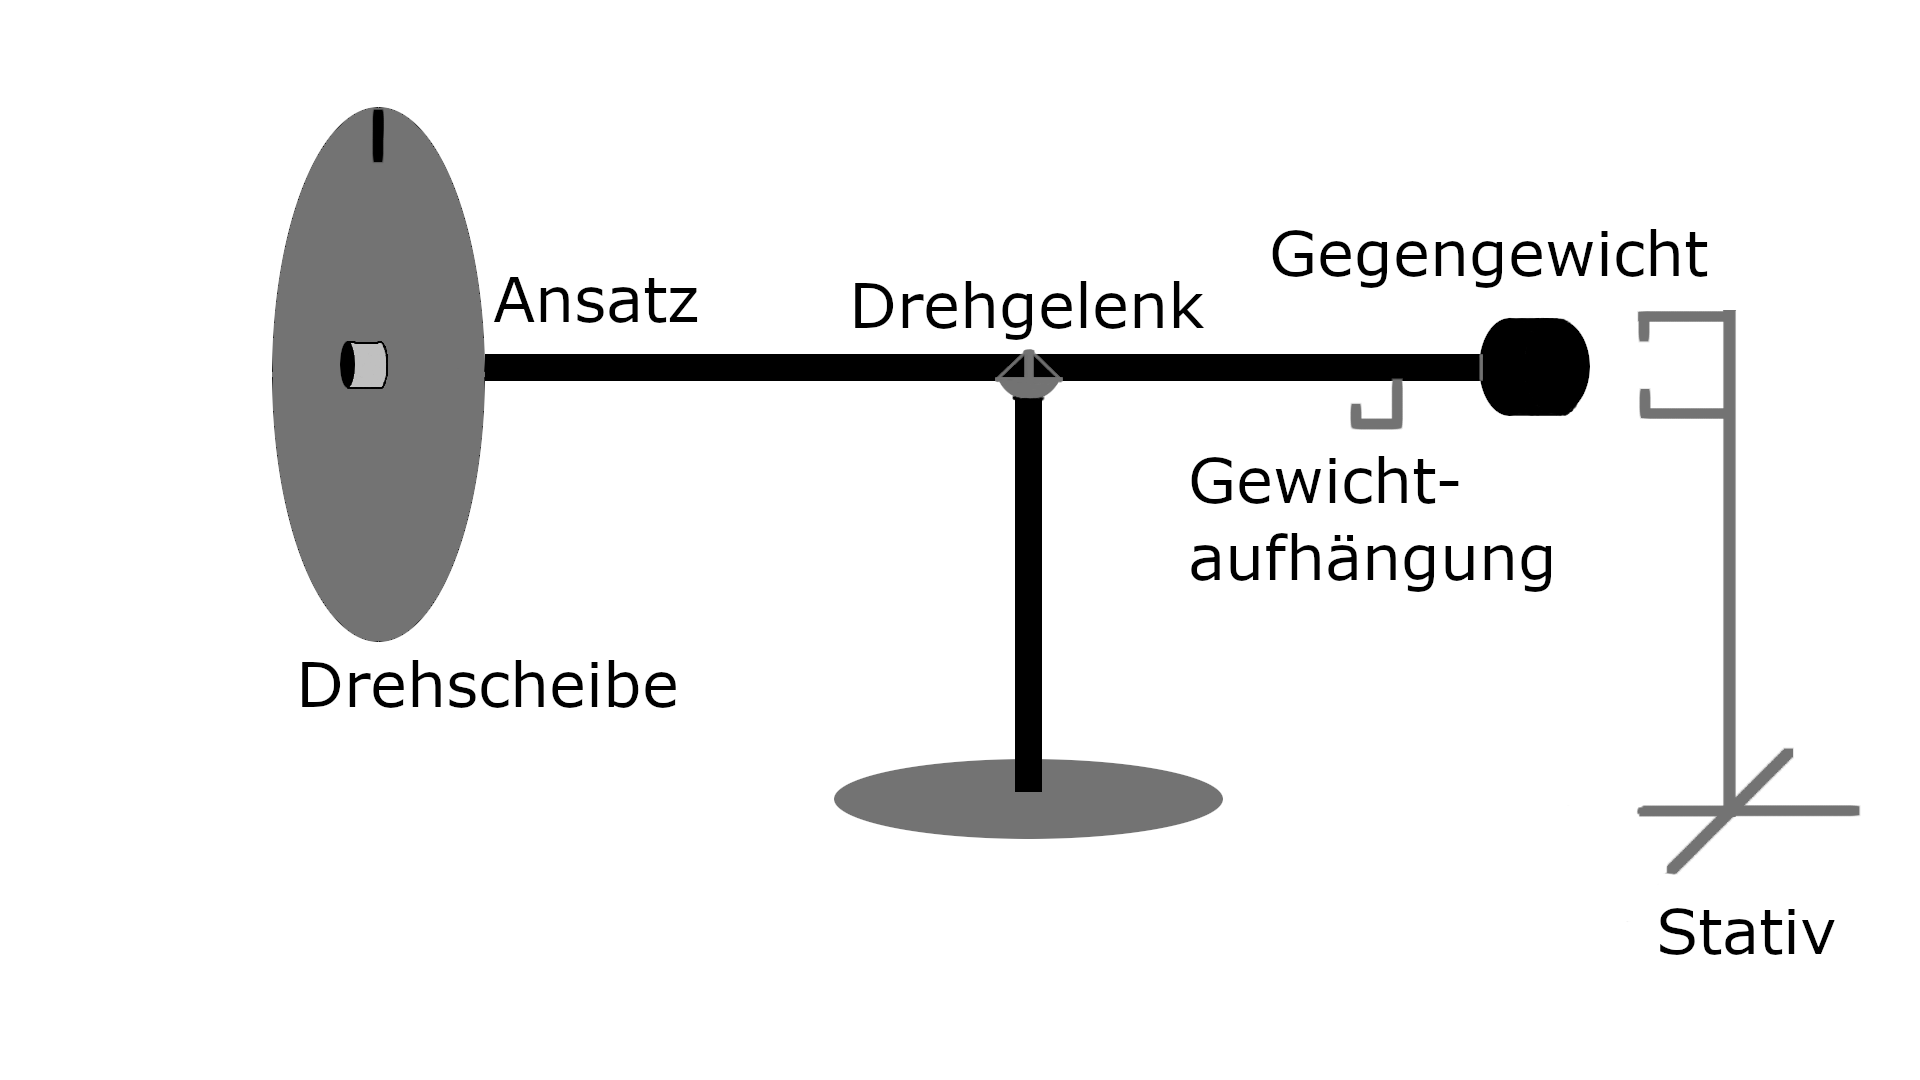
\includegraphics[width=\textwidth]{aufbau.png}
			\caption{Allgemeiner Versuchsaufbau}
		\end{figure}

	\section{Allgemeine Theorie}\label{Allgemeine_Theorie}
		Ein Trägheitsmoment ist der Zusammenhang zwischen der kinetischen Rotationsenergie eines Körpers und seiner Winkelgeschwindigkeit, nach der Formel \(K = \frac{1}{2}I \omega^2\).
		Damit stellt es den gleichen Zusammenhang her wie die Masse bei translatorischen Bewegungen. Die Formeln \(K = \frac{1}{2} m v^2\), sowie \(K = \frac{1}{2} I \omega^2 \) ähneln sich dabei stark.
		Das Trägheitsmoment kann man für diskrete oder kontinuierliche Masseverteilungen bestimmen.
		Für nur rotierende Körper ist die Summe aller Bewegungsenergien die gesamte Rotationsenergien. Zu einem diskreten Zeitpunkt lassen sich die Rotationen als geradlinige Bewegungen betrachten. Es gilt also:
		\begin{equation}
			K = \frac{1}{2} m_1 v_1^2 + \frac{1}{2} m_2 v_2^2 + \cdots = \sum \frac{1}{2} m_i v_i^2
		\end{equation}
		Wir ersetzen hier nun die Geschwindigkeit durch die Winkelgeschwindigkeit und den Radius (Abstand zur Drehachse) mit \(v = \omega r\)
		\begin{equation}
			K = \sum \frac{1}{2} m_i {\left( \omega r_i \right)}^2 = \frac{1}{2} \left( \sum m_i r_i^2 \right) \omega^2
		\end{equation} 
		Womit wir auf die Definition des Trägheitsmoments
		\begin{equation}\label{eq:trägheitsmoment_diskret}
			I = \sum m_i r_i^2
		\end{equation} kommen. Siehe~\cite{HallidayPhysik} \\
		Um ein solches Trägheitsmoment anzugeben braucht man aber zwingend noch eine dazugehörige Drehachse.
		Die Winkelgeschwindigkeiten und Radien in der Herleitung werden alle von der selben Achse aus angegeben.
		Bei krummen oder nicht symmetrischen Körpern kann man sich leicht visualisieren, dass ein verschieben der Achse einen großen Einfluss haben kann.
		Einen Stift entlang seiner langen Seite zu drehen fällt viel leichter, da die Masse des Stiftes nicht so weit von der Drehachse entfernt ist.
		Dreht man ihn um seine Spitze ist die Masse viel weiter von der Drehachse entfernt und das Trägheitsmoment damit merklich größer. % TODO: Bessere Bezeichnungen
		Natürlich kann man das Trägheitsmoment auch für volle Körper berechnen. Man braucht hierfür die Massenverteilung im Volumen. Die allgemeine Definition ist also:
		\begin{equation}
			I = \int_V \vec{r}_{\bot}^{\,2} \rho(\vec{r}) \,dV
		\end{equation}
		Man integriert über das gesamte Volumen mit der Dichteverteilung und den Abstandsquadraten. Diese Form ist der Grenzfall für unendlich viele Massestücke aus Definition~(\ref{eq:trägheitsmoment_diskret}).
		Hat man bereits ein Trägheitsmoment mit Drehachse durch den Massenmittelpunkt bestimmt, so lassen sich mit dem Steiner'schen Satz alle Trägheitsmoment von dazu parallel verschobenen Drehachsen berechnen.
		Man addiert dafür zu dem bereits bekannten Drehmoment \(I\) den Term \(m \cdot r^2\) hinzu (Siehe~\cite{Steiner}). Hieraus erkennt man sofort, dass das Drehmoment einer Achse die nicht 
		durch den Schwerpunkt geht, immer echt größer ist, da man nach der Regel des Steiner'schen Satzes etwas positives hinzuaddiert.
		Das Trägheitsmoment eines aus mehreren Teilkörpern zusammengesetzten Objekts lässt sich durch addieren der Teilträgheitsmomente zur gleichen Achse berechnen.
		Hier kann man das Trägheitsmoment eines Teilkörpers berechnen und dann mit Hilfe des Steiner'schen Satzes auf die richtige Achse verschieben.
		Dieser Eigenschaft ist sehr praktisch, da viele Trägheitsmomente bereits berechnet sind und sich in Refernztabellen, wie z.B. in Quelle~\cite{HallidayPhysik} finden lassen.
		Das Trägheitsmoment wird nicht nur für die Energieberechnung verwendet, sondern auch hier wieder ähnlich zur Masse, für den Drehimpuls \(L = I \omega \) und das Drehmoment \(M = I \alpha \).
		Trägheitsmomente eines Körpers lassen sich auch über einen Trägheitstensor ausdrücken, mit dessen Hilfe man das Trägheitsmoment zu jeder beliebigen Achse einfach berechnen lässt. \\
		Für die Intuition sei hier noch angefügt, dass je kleiner das Trägheitsmoment eines Körpers um eine Achse, desto leichter lässt er sich um sie drehen~\cite{HallidayPhysik}.

	\section{Trägheitsmoment über die Winkelbeschleunigung}

		\subsection{Durchführung}
			\begin{enumerate}
				\item Masse des Gewichts mit Faden \(m\) messen.
				\item Messen des Radius der Schnuraufwicklung (Zylindrischer Ansatz an der Vorderseite der Scheibe) mit der Schieblehre.
				\item Aufwickenln des Fadens und anhängen des Gewichts an die Kreisscheibe.
				\item Zeitmessung für Umdrehungen mit \enquote{Runden} Knopf von Smartphone Stoppuhr
			\end{enumerate} % TODO: Entweder oder
			Für diesen Versuch lassen wir auf die Scheibe ein konstantes Drehmoment wirken.
			Dies wird durch das Anhängen eines kleinen Gewichts der Masse \(m\) mit einer Schnur an einen hervorstehenden Zylinder erreicht.
			Die Schnur, an welcher das Gewicht hängt, wird auf diesen Zylinder aufgewickelt (Abb.~\ref{fig:Angehängte Masse}). \\
			Nun wird das Gewicht losgelassen, worauf hin das durch das Gewicht erzeugte Drehmoment die Scheibe in Rotation versetzt.
			Die Rotation wird durch das konstant wirkende Drehmoment weiter beschleunigt, sodass die Scheibe sich immer schneller dreht, also eine kürzere Zeit für jede Umdrehung braucht. \\
			Wir messen nun die Zeit \(t_R\), welche die Scheibe für eine Umdrehung benötigt.
			Eine Umdrehung der Scheibe erkennen wir daran, dass die Markierung wieder in ihre Ausgangslage zurück rotiert ist.
			Die Zeiten werden per Hand mit einer Handystoppuhr gemessen. Für jede Umdrehung messen wir mit der Rundenzeiten Funktion der Stoppuhr-App die Umdrehungszeit.
			Es werden so lange Zeiten gemessen, bis der Faden komplett abgewickelt ist. Es ist darauf zu achten, das das Gewicht nicht bereits wieder hoch gezogen wird und die Scheibe abbremst.
			Die Masse \(m\) wird mit einer Waage gemessen, wobei der Faden, mit dem sie Angehängt wird mitgewogen wird.
			Der Radius des Zylinders, an den die Masse angehängt wird, wird mit einer Schieblehre bestimmt.

			\begin{figure}
				\centering
				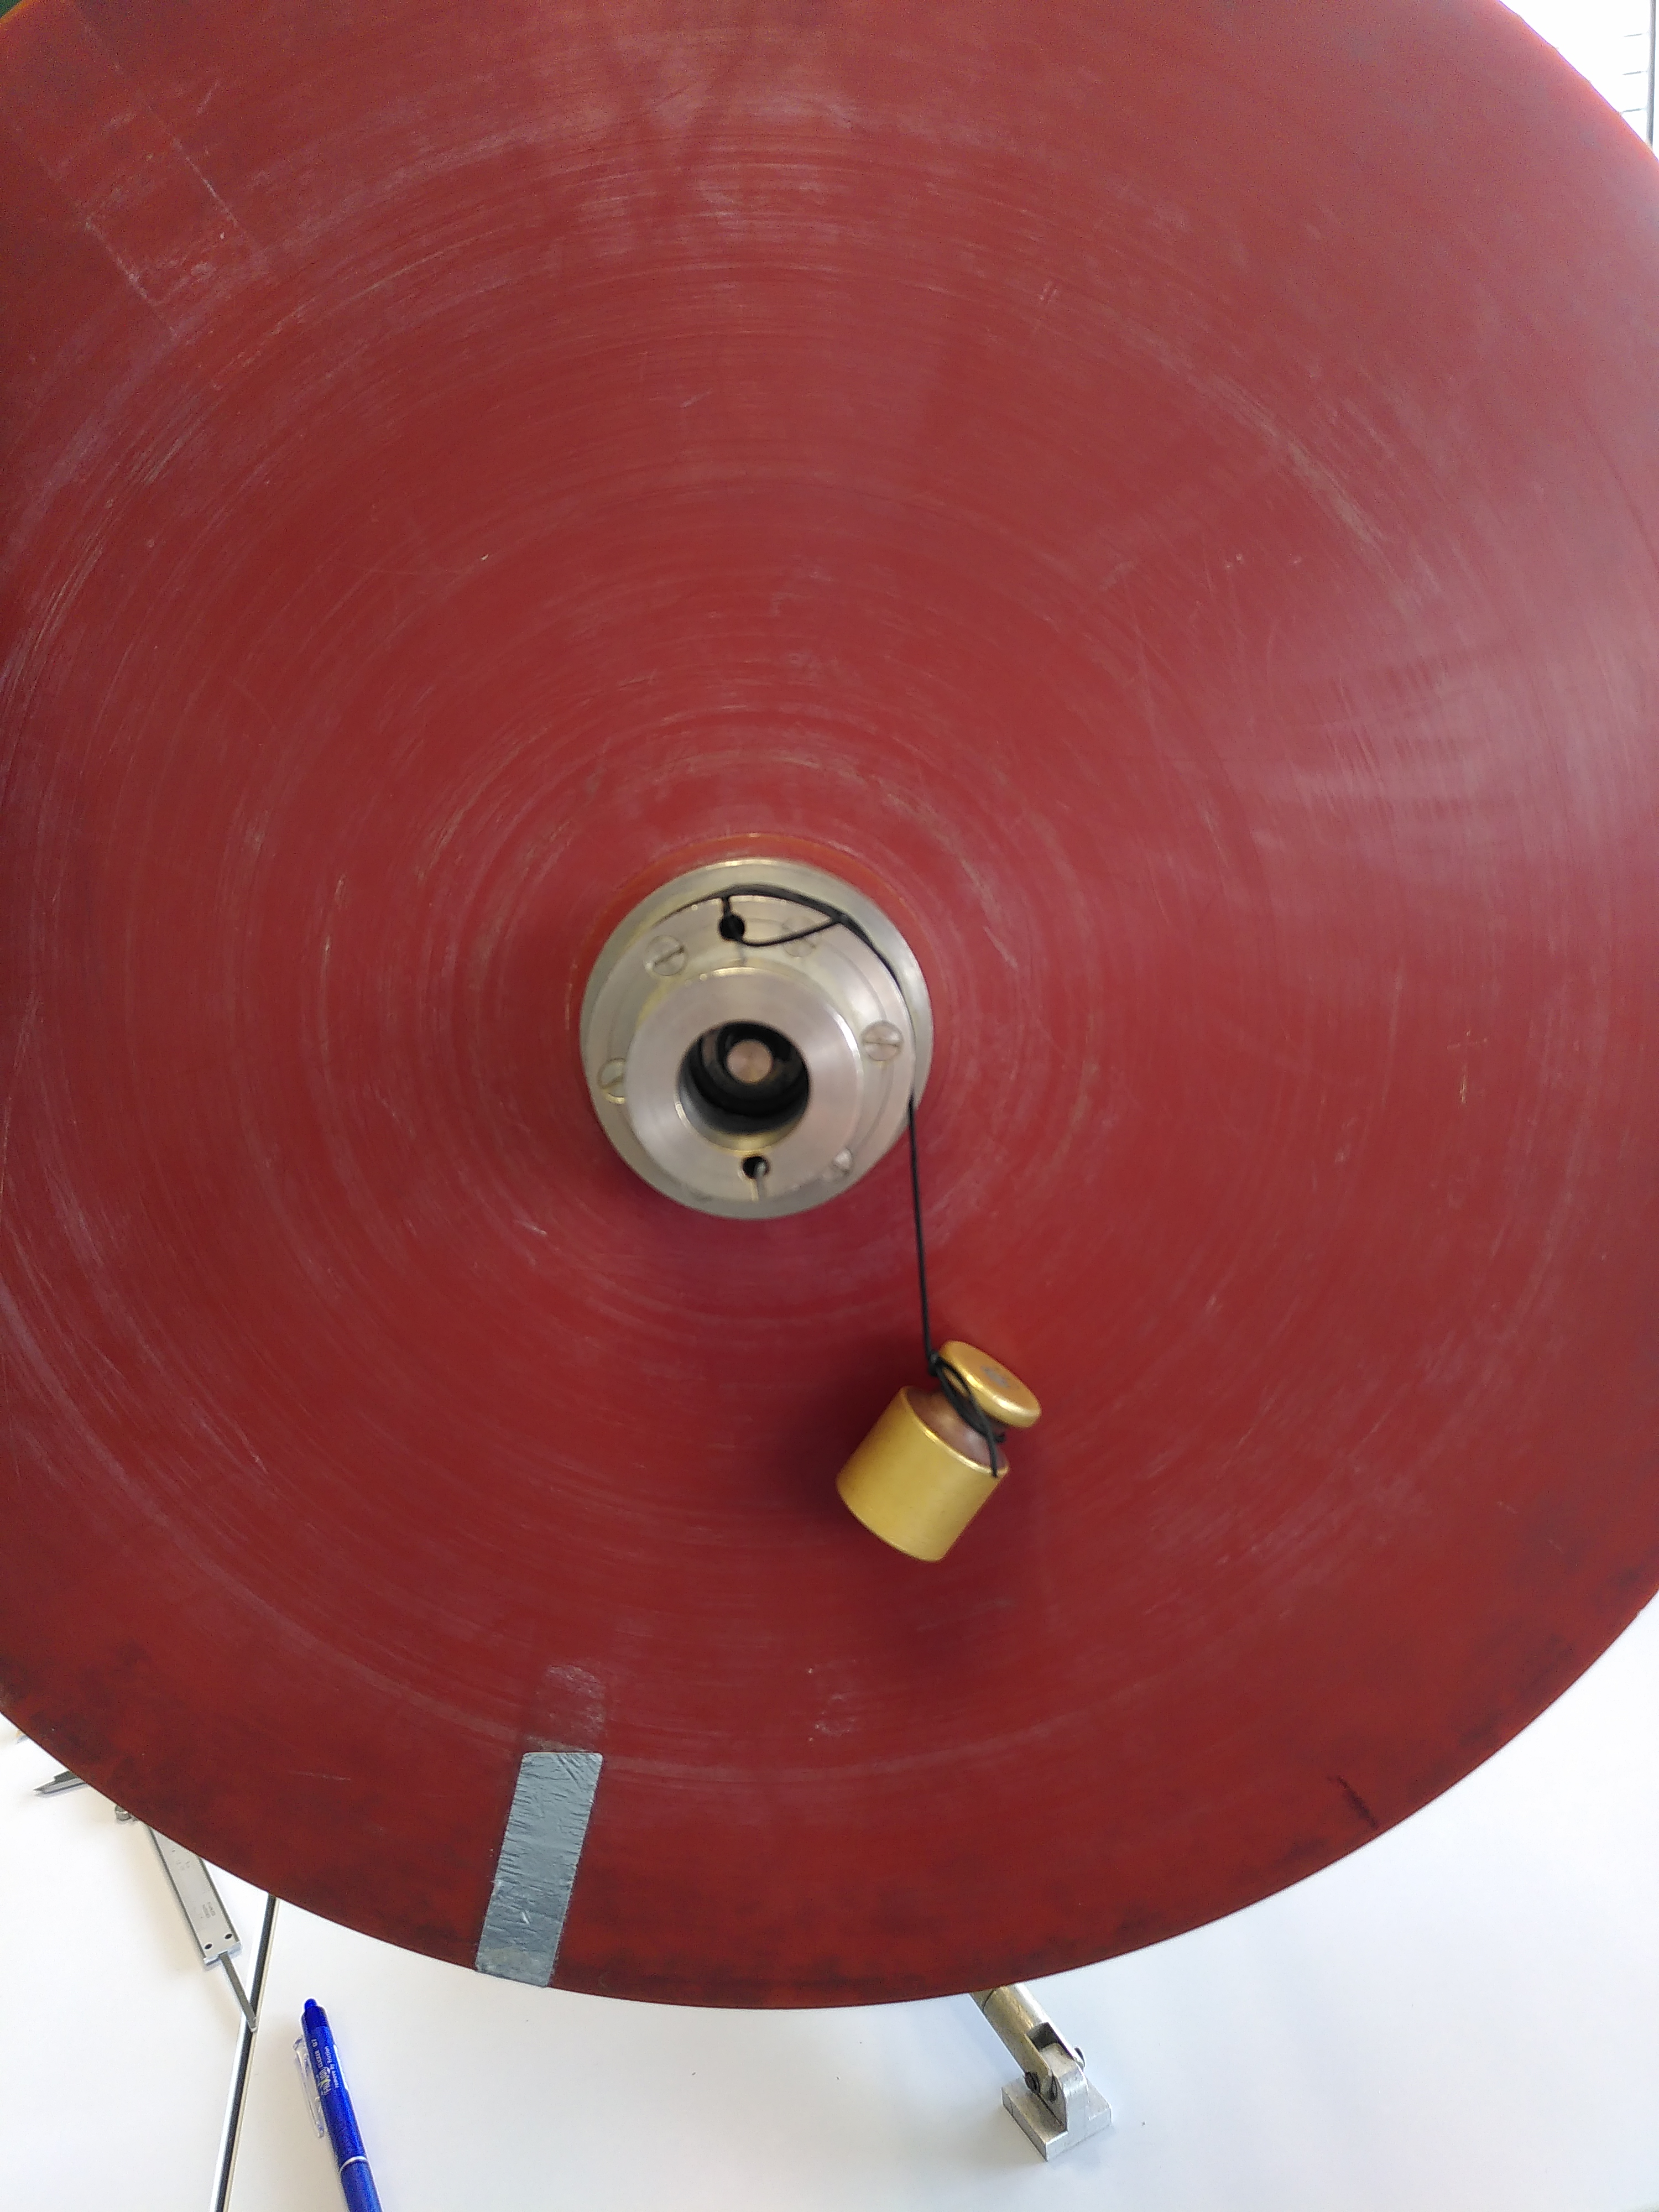
\includegraphics[width=0.5\textwidth]{Winkelbeschleunigung.jpg}
				\caption{\label{fig:Angehängte Masse}Die Masse angehängt an dem Zylinder}
			\end{figure}

		\subsection{Messergebnisse}
			Mit Hilfe der Waage wurde die Masse des kleinen Gewichts \(m\) auf \(\SI{99}{\gram}\) bestimmt.
			Die benutzte Waage hat eine Genauigkeit von einem Gramm.
			Die Schnuraufwicklung hat den Radius (Radius des Zylinders) \(r = \SI{4.93}{cm}\).
			Die dazu verwendete Schieblehre hat eine Genauigkeit von \(\SI{0.05}{mm}\) 
			Für die Messungen wurde eine Handystoppuhr verwendet mit einer Genauigkeit von einer Millisekunde.
			Der Winkel wurde mit dem Auge geschätzt. \\

			\subsubsection{Winkel und Zeiten}
				\begin{table}[!h]
					\centering
					\begin{tabular}{ | c | c | } 
						\hline
						Winkel \( \varphi \) & Rundenzeit \(t_R [\unit{\second}]\) \\
						\hline
						\( 2\pi \) & 4,89 \\
						\( 4\pi \) & 2,14 \\
						\( 6\pi \) & 1,67 \\
						\( 8\pi \) & 1,33 \\
						\( 10\pi \) & 1,21 \\
						\hline
					\end{tabular}
					\caption{Winkel und Rundenzeiten}
				\end{table}
				
				Damit ergibt sich für die Winkel und die insgesamt verstrichene Zeit:
				\begin{table}[!h]
					\centering
					\begin{tabular}{ | c | c | } 
						\hline
						\( \varphi \) & \(t [\unit{\second}]\) \\
						\hline
						\( 2\pi \) & 4,89 \\
						\( 4\pi \) & 7,03 \\
						\( 6\pi \) & 8,70 \\
						\( 8\pi \) & 10,03 \\
						\( 10\pi \) & 11,24 \\
						\hline
					\end{tabular}
					\caption{\label{tab:Winkel_Gesamtzeit}Winkel und Gesamtzeit}
				\end{table} \\
				Messwerte aus (\ref{fig:Messwerte1}).

		\subsection{Auswertung}
			\subsubsection{Formeln}
			Durch anhängen des Gewichts mit der Masse \(m\) auf den aufgewickelten Faden erzeugt man ein Drehmoment \(M = mgr\) wodurch die Scheibe eine konstante Winkelbeschleunigung erfährt.
			\begin{equation} \label{eq:Drehmoment}
				M = I \alpha = I \frac{d\omega}{dt}
			\end{equation} \(e\)
			Zwischen dem Winkel und der Winkelbeschleunigung \( \alpha \) besteht die Beziehung:
			\begin{equation} \label{eq:Beschleunigter_Winkel}
				\varphi = \frac{1}{2} \alpha t^2
			\end{equation}
			Sie gilt, wenn die Scheibe mit Winkelgeschwindigkeit und Winkel 0 beginnt \(\omega = \varphi = 0\).
			Hier gegeben, da die Scheibe zu Beginn des Experiments in Ruhe ist.
			Setzen wir die Formel~\ref{eq:Beschleunigter_Winkel} nach \( \alpha \) umgeformt in Formel~\ref{eq:Drehmoment} ein, so folgt:
			\begin{equation}
				I = \frac{M}{\alpha} = \frac{ Mt^2 }{2 \varphi}
			\end{equation}
			Das Drehmoment wird durch das am Faden hängende Gewicht erzeugt. Es erzeugt durch seine Aufhängung immer das Drehmoment \( M = mgr \). Setzen wir ein folgt:
			\begin{equation}
				I = \frac{ m g r \cdot t^2 }{ 2 \varphi }
			\end{equation}
			Hier können wir noch einen Teil durch die Steigung \(S = \frac{ \varphi }{ t^2 } \) ersetzen:
			\begin{equation}\label{eq:Trägheitsmoment_komplett}
				I = \frac{mgr}{2S}
			\end{equation}

			\subsubsection{Graphische Auswertung}
			% TODO: Gemaltes Bild einfügen
			In Gleichung (\ref{eq:Beschleunigter_Winkel}) erkennen wir den linearen Zusammenhang zwischen \( \varphi \) und \( t^2 \).
			Tragen wir also die gemessenen Werte für \( \varphi \) und \( t^2 \) in ein Koordinatensystem ein, sehen wir eine Gerade, weil die beiden Größen einfach proportional zueinander sind.
			Wir rechnen unsere Messwerte aus Tabelle~\ref{tab:Winkel_Gesamtzeit} um, indem wir die Zeiten quadrieren.
			\begin{center}
				\begin{tabular}{ | c | c | } 
					\hline
					\( \varphi \) & \(t^2 [\unit{\second^2}] \) \\
					\hline
					\( 2\pi \) & 23,91 \\
					\( 4\pi \) & 49,42 \\
					\( 6\pi \)  & 75,69 \\
					\( 8\pi \) & 100,60 \\
					\( 10\pi \) & 126,33 \\
					\hline
				\end{tabular}
			\end{center}
			Diese Werte werden in ein Diagramm eingetragen (Abbildung TODO:ref), und die Steigung \( S = \frac{\varphi}{t^2} \) wird bestimmt. Dazu werden zwei Punkte ausgewählt:
			\begin{equation}
				\begin{gathered}\label{eq:punkte}
					P_1: t^2_1 = 20s^2 ; \varphi_1 = 1,7 \pi \\
					P_2: t^2_2 = 130s^2 ; \varphi_2 = 10,3 \pi
				\end{gathered}
			\end{equation}
			Damit ergibt sich für \( S \):
			\begin{equation}
				S = \frac{ \varphi_2 - \varphi_1 }{ t^2_2 - t^2_2 } = \frac{ 10,3 \pi - 1,7 \pi }{ \SI{130}{\second^2} - \SI{20}{\second^2} } = \SI{0,2456}{\frac{1}{\second^2}}
			\end{equation}

			\subsubsection{Trägheitsmomentberechnung}
				Zur Berechnung des Ergebnisses setzen wir die Steigung \(S = \SI{0,2456}{\frac{1}{\second^2}} \), das Gewicht der beschleunigenden Masse \(m = \SI{99}{\gram} = \SI{0.099}{\kilogram}\), die Erdbeschleunigung
				\(g = \SI{9,81}{\frac{m}{s^2}} \), sowie den Radius der Aufhängung \(r = \SI{4.93}{cm} = \SI{0.0493}{\metre}\) in Gleichung (\ref{eq:Trägheitsmoment_komplett}) ein:
				\begin{equation}
					I = \frac{ \SI{0,099}{\kilogram} \cdot \SI{9,81}{\frac{m}{s^2}} \cdot \SI{0,0493}{m} }{ 2 \cdot \SI{0,2456}{\frac{1}{s^2}} } = \SI{0,0981}{\kilogram \cdot \metre^2}
				\end{equation}
			
			\subsubsection{Fehlerrechnung}
				Nun muss noch der maximale Fehler von \( I \) bestimmt werden, dieser ist gegeben als (Aufgabenstellung~\cite{AnleitungPraktikum}):
				\begin{equation}
					\Delta I = 
					\left| \frac{\partial I}{\partial m} \right| \Delta m +
					\left| \frac{\partial I}{\partial r} \right| \Delta r +
					\left| \frac{\partial I}{\partial S} \right| \Delta S
				\end{equation}
				Wir berechnen zunächst die partiellen Ableitungen von Gleichung \(\ref{eq:Trägheitsmoment_komplett}\):
				\begin{equation}
					\begin{aligned}
						\frac{\partial I}{\partial m} &= \frac{\partial}{\partial m} \frac{mgr}{2S} = \frac{gr}{2S} \\
						\frac{\partial I}{\partial r} &= \frac{\partial}{\partial r} \frac{mgr}{2S} = \frac{mg}{2S} \\
						\frac{\partial I}{\partial S} &= \frac{\partial}{\partial S} \frac{mgr}{2S} = -\frac{mgr}{2S^2} \\
					\end{aligned}
				\end{equation}
				Wir setzen die partiellen Ableitungen in die Formel ein:
				\begin{equation}
					\Delta I =
					\left| \frac{gr}{2S} \right| \Delta m +
					\left| \frac{mg}{2S} \right| \Delta r +
					\left| -\frac{mgr}{2S^2} \right| \Delta S
				\end{equation}

				\paragraph{Graphischer Fehler}
					Zunächst bestimmen wir \( \Delta S \), den Fehler für die graphische Darstellungen: % TODO: Ist Fehler für die Graphische Darstellung die richtige Bezeichnung?
					\begin{equation} % TODO: Wo kommt das her?
						\frac{\Delta S}{S} = \frac{ 2 \Delta t^2 }{t^2_2 - t^2_1}
					\end{equation}
					Wobei \( \Delta t^2 \) die größte Abweichung eines Messwertes von der Geraden bezeichnet.
					Bei unseren Messwerten ist das, das Wertepaar \( t = \SI{75,69}{\second} \); \( \varphi = 6\pi \).
					Hier weicht \( t^2 \) um \( \SI{1}{\second^2} \) von der gezeichneten Geraden ab. % TODO: Wie wurde die Gerade gezeichnet
					Mit \( t^2_1 \), \( t^2_2 \) von \( P_1 \) und \( P_2 \) (\ref{eq:punkte}) beträgt der Fehler von \( S \):
					\begin{equation}
						\Delta S = \frac{2\cdot 1s^2}{130s^2 - 20s^2}0,2456\frac{1}{s^2} = 0,0045\frac{1}{s^2}
					\end{equation}
				
				\paragraph{Maximaler Fehler}
					Der maximale Fehler der Waage, mit welcher \(m\) bestimmt wurde beträgt \(\Delta m = \SI{1}{\gram} = \SI{0.001}{\kilogram}\),
					und der Fehler der Schieblehre liegt bei \( \Delta r = \SI{0,05}{mm} = \SI{5e-5}{\metre} \).
					Somit ergibt sich für \( \Delta I \), mit einsetzen aller Messfehler und Variablen:
					\begin{equation}
						\begin{aligned}
							\Delta I =& \left| \frac{ \SI{9,81}{\frac{\metre}{\second^2}} \cdot \SI{0,0493}{\metre} }{ 2 \cdot \SI{0,2456}{\frac{1}{\second^2}} } \right| \cdot \SI{0,001}{\kilogram}\\
							+& \left| \frac{ \SI{0,099}{\kilogram} \cdot \SI{9,81}{\frac{\metre}{\second^2}} }{ 2 \cdot \SI{0,2456}{\frac{1}{\second^2}} } \right| \cdot \SI{5e-5}{\metre} \\
							+& \left| - \frac{ \SI{0,099}{\kilogram} \cdot  \SI{9,81}{\frac{\metre}{\second^2}} \cdot \SI{0,0493}{\metre} }{ 2 \cdot {(\SI{0,2456}{\frac{1}{\second^2}})}^2 } \right| \cdot \SI{0,0045}{\frac{1}{s^2}} \\
							=& \SI{3,76e-3}{ \kilogram \cdot \metre^2 }
						\end{aligned}
					\end{equation}

			\subsubsection{Endergebnis}
				Das Trägheitsmoment beträgt bei der Bestimmung über die Winkelbeschleunigung also:
				\begin{equation}
					I = \SI{9,81e-2}{ \kilogram \cdot \metre^2 } \pm \SI{0,376e-2}{ \kilogram \cdot \metre^2 }
				\end{equation}

	\section{Trägheitsmoment über die Schwingungsdauer einer Pendelbewegung}
		\subsection{Durchführung}
			\begin{enumerate}
				\item Masse des Gewichts \(m\) messen.
				\item Messen des Abstands \(R\) zwischen dem Gewicht und dem Mittelpunkt der Scheibe.
				\item Scheibe unter kleinem Winkel auslenken
				\item Zeitmessung für zehn Perioden mit Handystoppuhr messen
			\end{enumerate} % TODO: Entweder oder
			Für diesen Versuch befestigen wir ein kleines Gewicht mit der Masse \(m\) am äußeren Rand der Scheibe.
			Durch diese weitere Masse ist die Masseverteilung nicht mehr gleichmäßig auf der gesamten Scheibe. Der Schwerpunkt wird in Richtung Rand, weg von der Drehachse verschoben.
			Dadurch dreht sich die Scheibe nicht mehr um eine Achse die durch den Schwerpunkt geht.
			Im untersten Punkt ist die Masse in Ruhe, lenkt man sie aus, dreht also an der Scheibe wirkt ein Drehmoment, das die Scheibe wieder in die Ausgangslage zurück drehen möchte.
			Dieses rücktreibende Drehmoment hängt vom Auslenkungswinkel ab und kann für kleine Winkel (Kleinwinkelnäherung) als harmonische Schwingung betrachtet werden.
			Über die Periodendauer der Pendelbewegung, die Masse und ihren Abstand zum Mittelpunkt können wir das Drehmoment der Scheibe berechnen.

			\begin{figure}[!h]
				\centering
				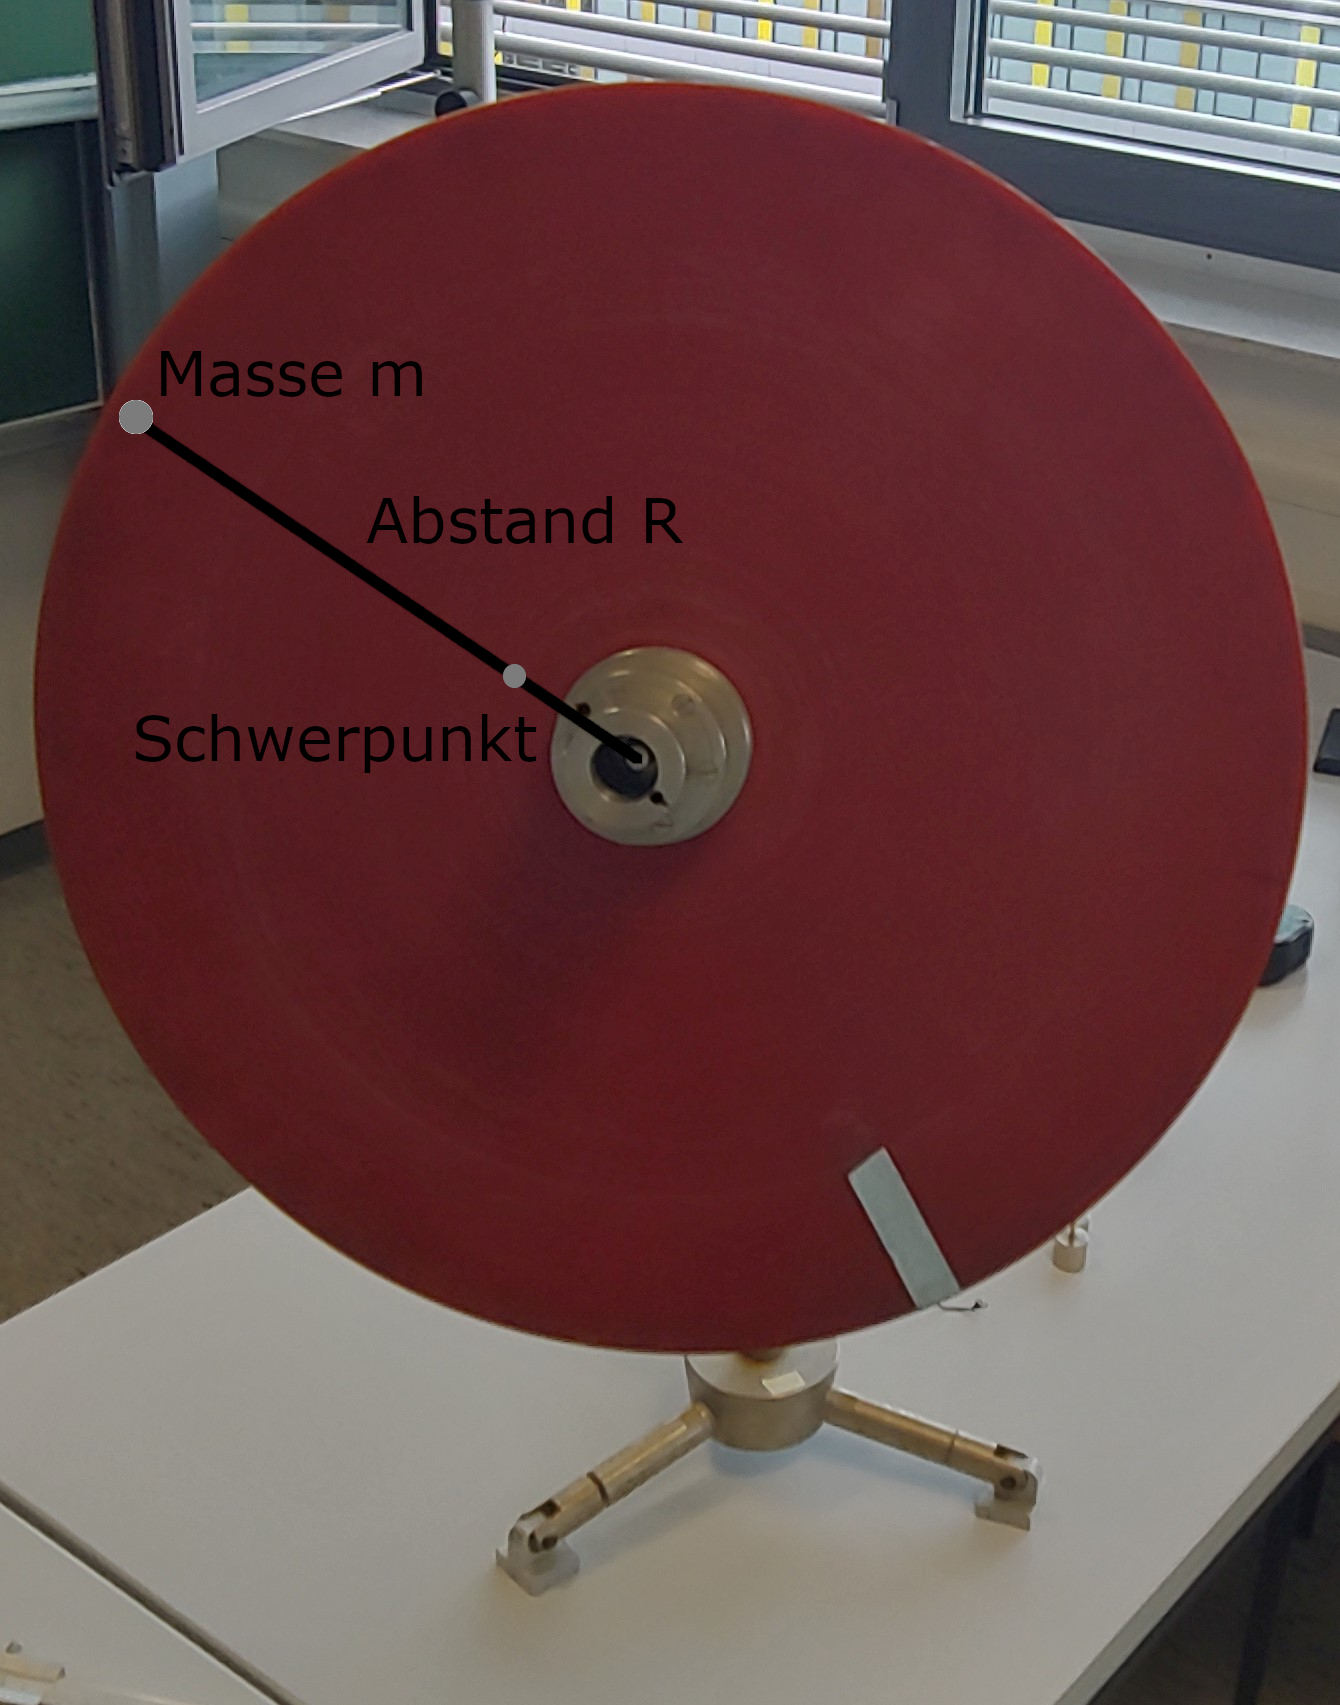
\includegraphics[width=0.5\textwidth]{schwingung_aufbau.png}
				\caption{\label{fig:Schwingung_Aufbau}Der Versuchsaufbau mit relevanten Größen}
			\end{figure}

		\subsection{Messergebnisse}
			Das Gewicht das außen an der Scheibe angebracht wird, wurde mit Hilfe einer Waage auf \(\SI{101}{\gram}\) bestimmt.
			Die benutzte Waage hat eine Genauigkeit von einem Gramm.
			Der Abstand \(R\) (Siehe Abbildung~\ref{fig:Schwingung_Aufbau}) vom Mittelpunkt der Scheibe
			bis zum angehängten Gewicht beträgt \(\SI{18,7}{cm}\).
			Das dazu verwendete Maßband hat eine Genauigkeit von einem Millimeter. \\
			Die Schwingungsdauer wurde für zehn Perioden mit \(\SI{32,04}{\second}\) gemessen.
			Die Handystoppuhr die für die Zeitmessung verwendet wurde hat eine Genauigkeit von einer Millisekunde.
			
		\subsection{Auswertung}

			\subsubsection{Formeln}
				Das Trägheitsmoment der Scheibe, \(I\) wird durch anbringen der Masse \(m\) verändert.
				Das Trägheits\-moment \(I\) bezieht sich auf die Achse die durch den Mittelpunkt und Schwerpunkt der Scheibe geht.
				Die kleine Masse verschiebt den Schwerpunkt nach außen (Siehe~\ref{fig:Schwingung_Aufbau}).
				Das neue Trägheitsmoment von Scheibe und Masse gemeinsam nennen wir \(I'\). Dieses können wir mit dem Steiner'schen Satz berechnen (Quelle~\cite{ExPhy1}).
				\begin{equation}\label{eq:Neues_Trägheismoment}
					I' = I + m \cdot R^2
				\end{equation}
				Wie wir bereits im Kapitel~\ref{Allgemeine_Theorie} in Gleichung~(\ref{eq:trägheitsmoment_diskret}) gesehen haben, steuert eine weitere diskrete Masse den Anteil \( m_i r_i^2\)
				zum Trägheitsmoment dazu. Hier \( m \cdot R^2\).
				Das Trägheitsmoment \(I'\) ist zur Achse des Drehmoments \(I\) parallel nach außen, in Richtung der kleinen Masse, verschoben.
				Die Achse des Trägheitsmoments \(I'\) geht jedoch nicht durch den neuen Schwerpunkt, da sonst das System nicht schwingen würde. \\ % TODO: ???
				Da die Achse nun nicht mehr durch den Schwerpunkt geht, gibt es ein Direktionsmoment. Es hat die selbe physikalische Bedeutung wie die rücktreibenden Kraft beim Federpendel.
				Das durch die Masse erzeugte Drehmoment ist: \(M = R \times \vec{F}\), da wir aber nur mit Beträgen rechnen folgt:
				\begin{equation}
					|\vec{M}| = M = R \cdot F \cdot \sin \varphi
				\end{equation}
				Die Kraft ist hier die Gewichtskraft der kleinen Masse also \(F = m \cdot g\). Zusammen:
				\begin{equation}
					M = R \cdot m \cdot g \cdot \sin \varphi
				\end{equation}
				Das Direktionsmoment ist definiert als \(D = \frac{M}{\varphi}\), also rücktreibendes Drehmoment pro Winkeleinheit:
				\begin{equation}
					D = \frac{M}{\varphi} = \frac{ R \cdot m \cdot g \cdot \sin \varphi }{ \varphi }
				\end{equation}
				Lenken wir nur kleine Winkel aus können wir für das Direktionsmoment die Kleinwinkelnäherung (Taylorentwicklung von \( \sin \varphi \) abgebrochen nach der ersten Ordnung)
				anwenden. Wir ersetzen also \( \sin \varphi \) mit \( \varphi \). Im Experiment wurde auf Grund dieser Näherung die Scheibe nur um einen kleinen Winkel ausgelenkt.
				\begin{equation}\label{eq:Genähertes_Direktionsmoment}
					D = \frac{ R \cdot m \cdot g \cdot \sin \varphi }{ \varphi } \approx \frac{ R \cdot m \cdot g \cdot \varphi }{ \varphi } = R \cdot m \cdot g
				\end{equation}
				% TODO: Aufstellen DGL mit MMdP Skript Seite 109
				Für ein Pendel mit Direktionsmoment gilt für die Schwingungsdauer:
				\begin{equation}
					T = 2 \pi \sqrt{ \frac{I'}{D} }
				\end{equation}
				Setzen wir für \(I'\) und \(D\) die in den Formeln (\ref{eq:Neues_Trägheismoment}) und (\ref{eq:Genähertes_Direktionsmoment}) ein, erhalten wir die folgende Formel:
				\begin{equation}
					T = 2 \pi \sqrt{ \frac{ I + m \cdot R^2 }{ R \cdot m \cdot g } }
				\end{equation}
				Im letzten Schritt formen wir die Gleichung nach dem zu bestimmenden Trägheitsmoment \(I\) um:
				\begin{equation}
					\begin{gathered} \label{eq:Trägheitsmoment_Schwingung}
						T = 2 \pi \sqrt{ \frac{ I + m \cdot R^2 }{ m \cdot g \cdot R } } \Leftrightarrow \\
						\frac{T}{ 2 \pi } = \sqrt{ \frac{ I + m \cdot R^2 }{ m \cdot g \cdot R } } \Leftrightarrow \\
						{\left( \frac{T}{ 2 \pi } \right)}^2 = \frac{ I + m \cdot R^2 }{ m \cdot g \cdot R } \Leftrightarrow \\
						\frac{T^2}{4 \pi^2} \cdot m \cdot g \cdot R = I + m \cdot R^2 \Leftrightarrow \\
						\frac{T^2}{4 \pi^2} \cdot m \cdot g \cdot R - m \cdot R^2 = I \Leftrightarrow \\
						I = R \cdot m \cdot \left( \frac{T^2 \cdot g }{ 4 \pi^2 } - R \right)
					\end{gathered}
				\end{equation}
				Einheitenkontrolle:
				\begin{equation}
					[I] = \unit{\metre} \cdot \unit{\kilogram} \cdot \left( \unit{\second^2} \cdot \unit{\frac{\metre}{\second^2}} - \unit{\metre} \right) = \unit{\kilogram \cdot \metre^2}
				\end{equation}

			\subsubsection{Trägheitsmomentberechnung}
				Gemessen wurden im Experiment zehn Periodendauern. Da bei einer harmonischen Schwingung die Periodendauer nicht von der Auslenkung abhängt und hier also konstant ist, teilen wir unseren gemessenen Wert durch zehn:
				\begin{equation}
					T = \frac{ \SI{32,04}{\second} }{ 10 } = \SI{3,204}{\second}
				\end{equation}
				Zur Berechnung des Ergebnisses setzen wir die Erdbeschleunigung \(\SI{9,81}{\frac{\metre}{\second^2}}\), die kleine Masse \(m = \SI{101}{\gram} = \SI{0,101}{\kilogram} \),
				den Abstand \(R = \SI{18,7}{cm} = \SI{0,187}{\metre} \), sowie die Periodendauer \( T = \SI{3,204}{\second} \) in Formel (\ref{eq:Trägheitsmoment_Schwingung}) ein:
				\begin{equation}
					I = \SI{0,187}{\metre} \cdot \SI{0,101}{\kilogram} \cdot \left( \frac{ {( \SI{3,204}{\second} )}^2 \cdot \SI{9,81}{\frac{\metre}{\second^2}} }{ 4 \pi^2 } - \SI{0,187}{\metre} \right) = \SI{0,0446}{\kilogram \cdot \metre^2}
				\end{equation}
				% 0.187 metre * 0.101 kilogram * ( ((3.203 seconds)^2 * 9.81 metres per second squared )/(4 pi^2) - 0.187 metre)

			\subsubsection{Fehlerrechnung}
				Wie in Teilversuch 1 berechnen wir den maximalen Fehler:
				\begin{equation}
					\Delta I = 
					\left| \frac{\partial I}{\partial m} \right| \Delta m +
					\left| \frac{\partial I}{\partial R} \right| \Delta R +
					\left| \frac{\partial I}{\partial T} \right| \Delta T
				\end{equation}
				Dazu berechnen wir die partiellen Ableitungen von Gleichung (\ref{eq:Trägheitsmoment_Schwingung}):
				\begin{equation}
					\begin{aligned}
						\frac{\partial I}{\partial m} &= \frac{\partial}{\partial m} \left( \frac{T^2}{4 \pi^2} \cdot m \cdot g \cdot R - m R^2 \right) = \frac{T^2}{4 \pi^2} \cdot g \cdot R - R^2 \\
						\frac{\partial I}{\partial R} &= \frac{\partial}{\partial R} \left( \frac{T^2}{4 \pi^2} \cdot m \cdot g \cdot R - m R^2 \right) = \frac{T^2}{4 \pi^2} \cdot m \cdot g - 2 m R = m \cdot \left( \frac{T^2 \cdot g }{4 \pi^2} - 2R \right) \\
						\frac{\partial I}{\partial T} &= \frac{\partial}{\partial T} \left( \frac{T^2}{4 \pi^2} \cdot m \cdot g \cdot R - m R^2 \right) = \frac{T}{2 \pi^2} \cdot m \cdot g \cdot R  = \frac{T \cdot m \cdot g \cdot R}{2 \pi^2 } \\
					\end{aligned}
				\end{equation}
				Wir setzen die partiellen Ableitungen in die Formel für den maximalen Fehler ein:
				\begin{equation}\label{eq:Maximaler_Fehler_Schwingung}
					\Delta I = 
					\left| \frac{T^2}{4 \pi^2} \cdot g \cdot R - R^2 \right| \Delta m +
					\left| m \cdot \left( \frac{T^2 \cdot g }{4 \pi^2} - 2R \right) \right| \Delta R +
					\left| \frac{T \cdot m \cdot g \cdot R}{2 \pi^2 } \right| \Delta T
				\end{equation}
				Der Fehler der Abstandsmessung \(\Delta R\) wäre allein vom Maßband \(\SI{1}{mm}\).
				Wegen des Zylindrischen Ansatzes auf der Vorderseite der Scheibe lässt sich der Abstand aber mitnichten so genau messen.
				Wir setzen hier einen Fehler von \(\SI{5}{mm} = \SI{0,005}{\metre} \) an. \\
				Der Messfehler der Waage ist \(\Delta m = \SI{1}{\gram}\). \\
				Die Auflösung der für den Versuch verwendeten Stoppuhr (Handystoppuhr) ist eine \(\SI{1}{ms}\).
				Die menschliche Reaktionszeit beträgt aber bereits \(\approx \SI{180}{ms} \) (Siehe~\cite{Reaktionszeit})
				Gestoppt wurde am Umkehrpunkt der Pendelschwingung, wobei diese mit bloßem Auge beobachtet wurde, was das Ergebnis weiter verfälscht.
				Bis dann die Stoppuhr gedrückt wurde sind bereits \(\approx \SI{0,2}{\second}\) vergangen.
				Da die gleiche Verzögerung auch beim Beginn der Messung entsteht, schätzen wir den Messfehler auf \(\SI{0,25}{\second}\).
				Deutlich genauere Messwerte wären mit Hilfe von Videoanalyse zu bekommen, wobei der Messfehler hier die Framerate des Videos wäre.
				Der Messfehler bezieht sich aber auf zehn Periodendauern weshalb wir die Unsicherheit hier noch einmal durch zehn teilen:
				\begin{equation}
					\Delta T = \frac{\SI{0,25}{\second}}{10} = \SI{0,025}{\second}
				\end{equation} 
				Wir setzen nun die Messfehler \( \Delta m = \SI{0,001}{\kilogram} \), \( \Delta R = \SI{0,005}{\metre} \) und \(\Delta T = \SI{0,025}{\second} \), sowie alle weiteren gemessenen Größen und Variablen
				\(g = \SI{9,81}{\frac{\metre}{\second^2}} \), \(m = \SI{0,101}{\kilogram} \), \(R = \SI{0,187}{\metre} \) und \( T = \SI{3,204}{\second} \) in Gleichung~(\ref{eq:Maximaler_Fehler_Schwingung}) ein:
				\begin{equation}
					\begin{aligned}
						\Delta I &= \\
						&\left| \frac{ {\SI{3,204}{\second}}^2 }{4 \pi^2} \cdot \SI{9,81}{\frac{\metre}{\second^2}} \cdot \SI{0,187}{\metre} - {\left(\SI{0,187}{\metre}\right)}^2 \right| \cdot \SI{0,001}{\kilogram} + \\
						&\left| \SI{0,101}{\kilogram} \cdot \left( \frac{ {\SI{3,204}{\second}}^2 \cdot \SI{9,81}{\frac{\metre}{\second^2}} }{4 \pi^2} - 2 \cdot \SI{0,187}{\metre} \right) \right| \cdot \SI{0,005}{\metre} + \\
						&\left| \frac{ \SI{3,204}{\second} \cdot \SI{0,101}{\kilogram} \cdot \SI{9,81}{\frac{\metre}{\second^2}} \cdot \SI{0,187}{\metre} }{2 \pi^2 } \right| \cdot \SI{0,025}{\second} \\
						&= \SI{0.002293}{ \kilogram \cdot \metre^2 }
					\end{aligned}
				\end{equation}
				% abs((3.204s)^2/(4*pi^2)*9.81m/s^2 *0.187m - (0.187m)^2 ) * 0.001kg + abs( 0.101kg * ((3.204s)^2 * 9.81m/s^2 /(4*pi^2) - 2*0.187 m)) * 0.005m + abs((3.204s*0.101kg* 9.81m/s^2* 0.187m)/(2*pi^2))*0.025s
				In diesem maximalen Fehler bleibt die Kleinwinkelnäherung unberücksichtigt etc.

			\subsubsection{Endergebnis}
				Das Trägheitsmoment beträgt bei der Bestimmung über eine Pendelbewegung also:
				\begin{equation}
					I = \SI{4,46e-2}{ \kilogram \cdot \metre^2 } \pm \SI{0,229e-2}{ \kilogram \cdot \metre^2 }
				\end{equation}


	\section{Trägheitsmoment über eine Präzessionsbewegung}
		\subsection{Durchführung}

		\subsection{Messergebnisse}
		
		\subsection{Auswertung}

	\section{Fazit}
		Versuch 1 graphische Auswertung, nicht rein mathematisch

		TODO: Welcher Versuch ist am Besten geeignet, am einfachsten, am genausten, etc... um das Trägheitsmoment zu bestimmen.
		Vergleich der Ergebnisse
		Hoffentlich ähnliche Ergebnisse.
		Diskutiere z.B Reibungseffekte, Kleinwinkelnäherung, etc.
		Fazit beste Methode, z.B. kleinster Fehler, Durchführung am wenigsten Aufpassen.
		Direkt bestimmen mit Gewicht und Radius


	\printbibliography[title={Quellen}]

	\begin{figure}[!h]\label{fig:Messwerte1}
		\centering
		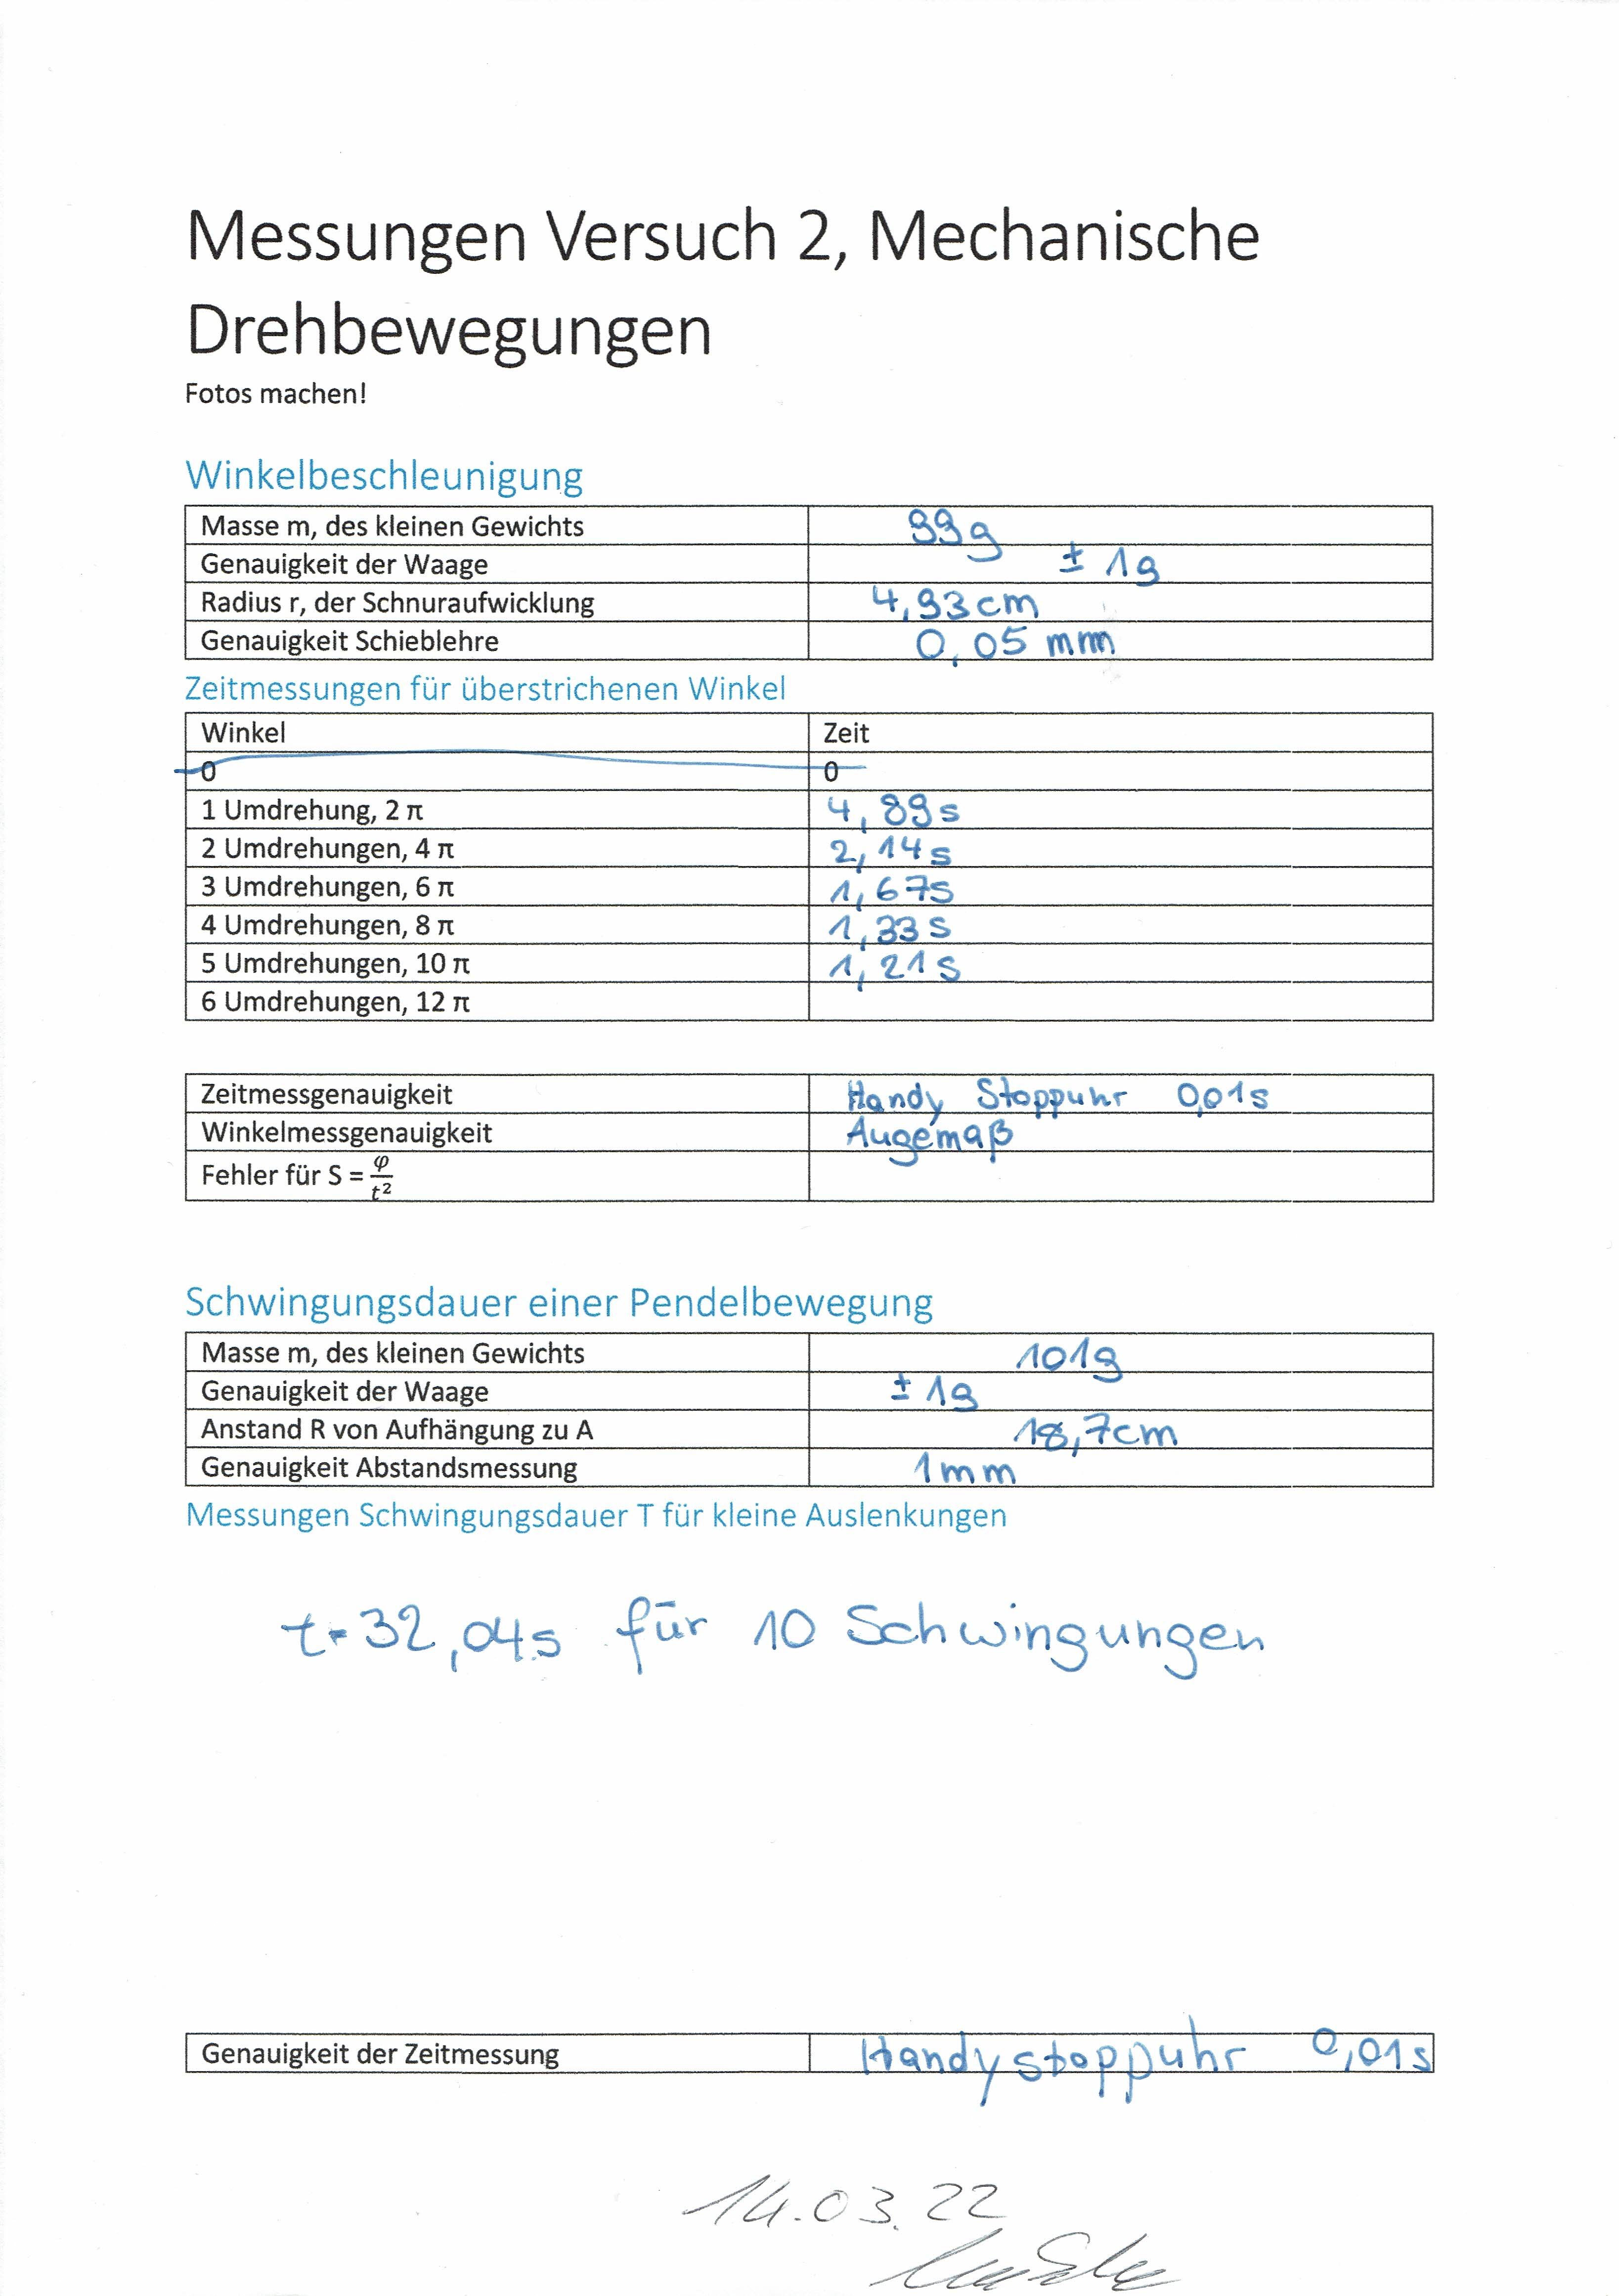
\includegraphics[height=14cm]{messwerte1.jpg}
		\caption{Messwerte der ersten beiden Teilversuche}
	\end{figure}

	\begin{figure}[!h]\label{fig:Messwerte2}
		\centering
		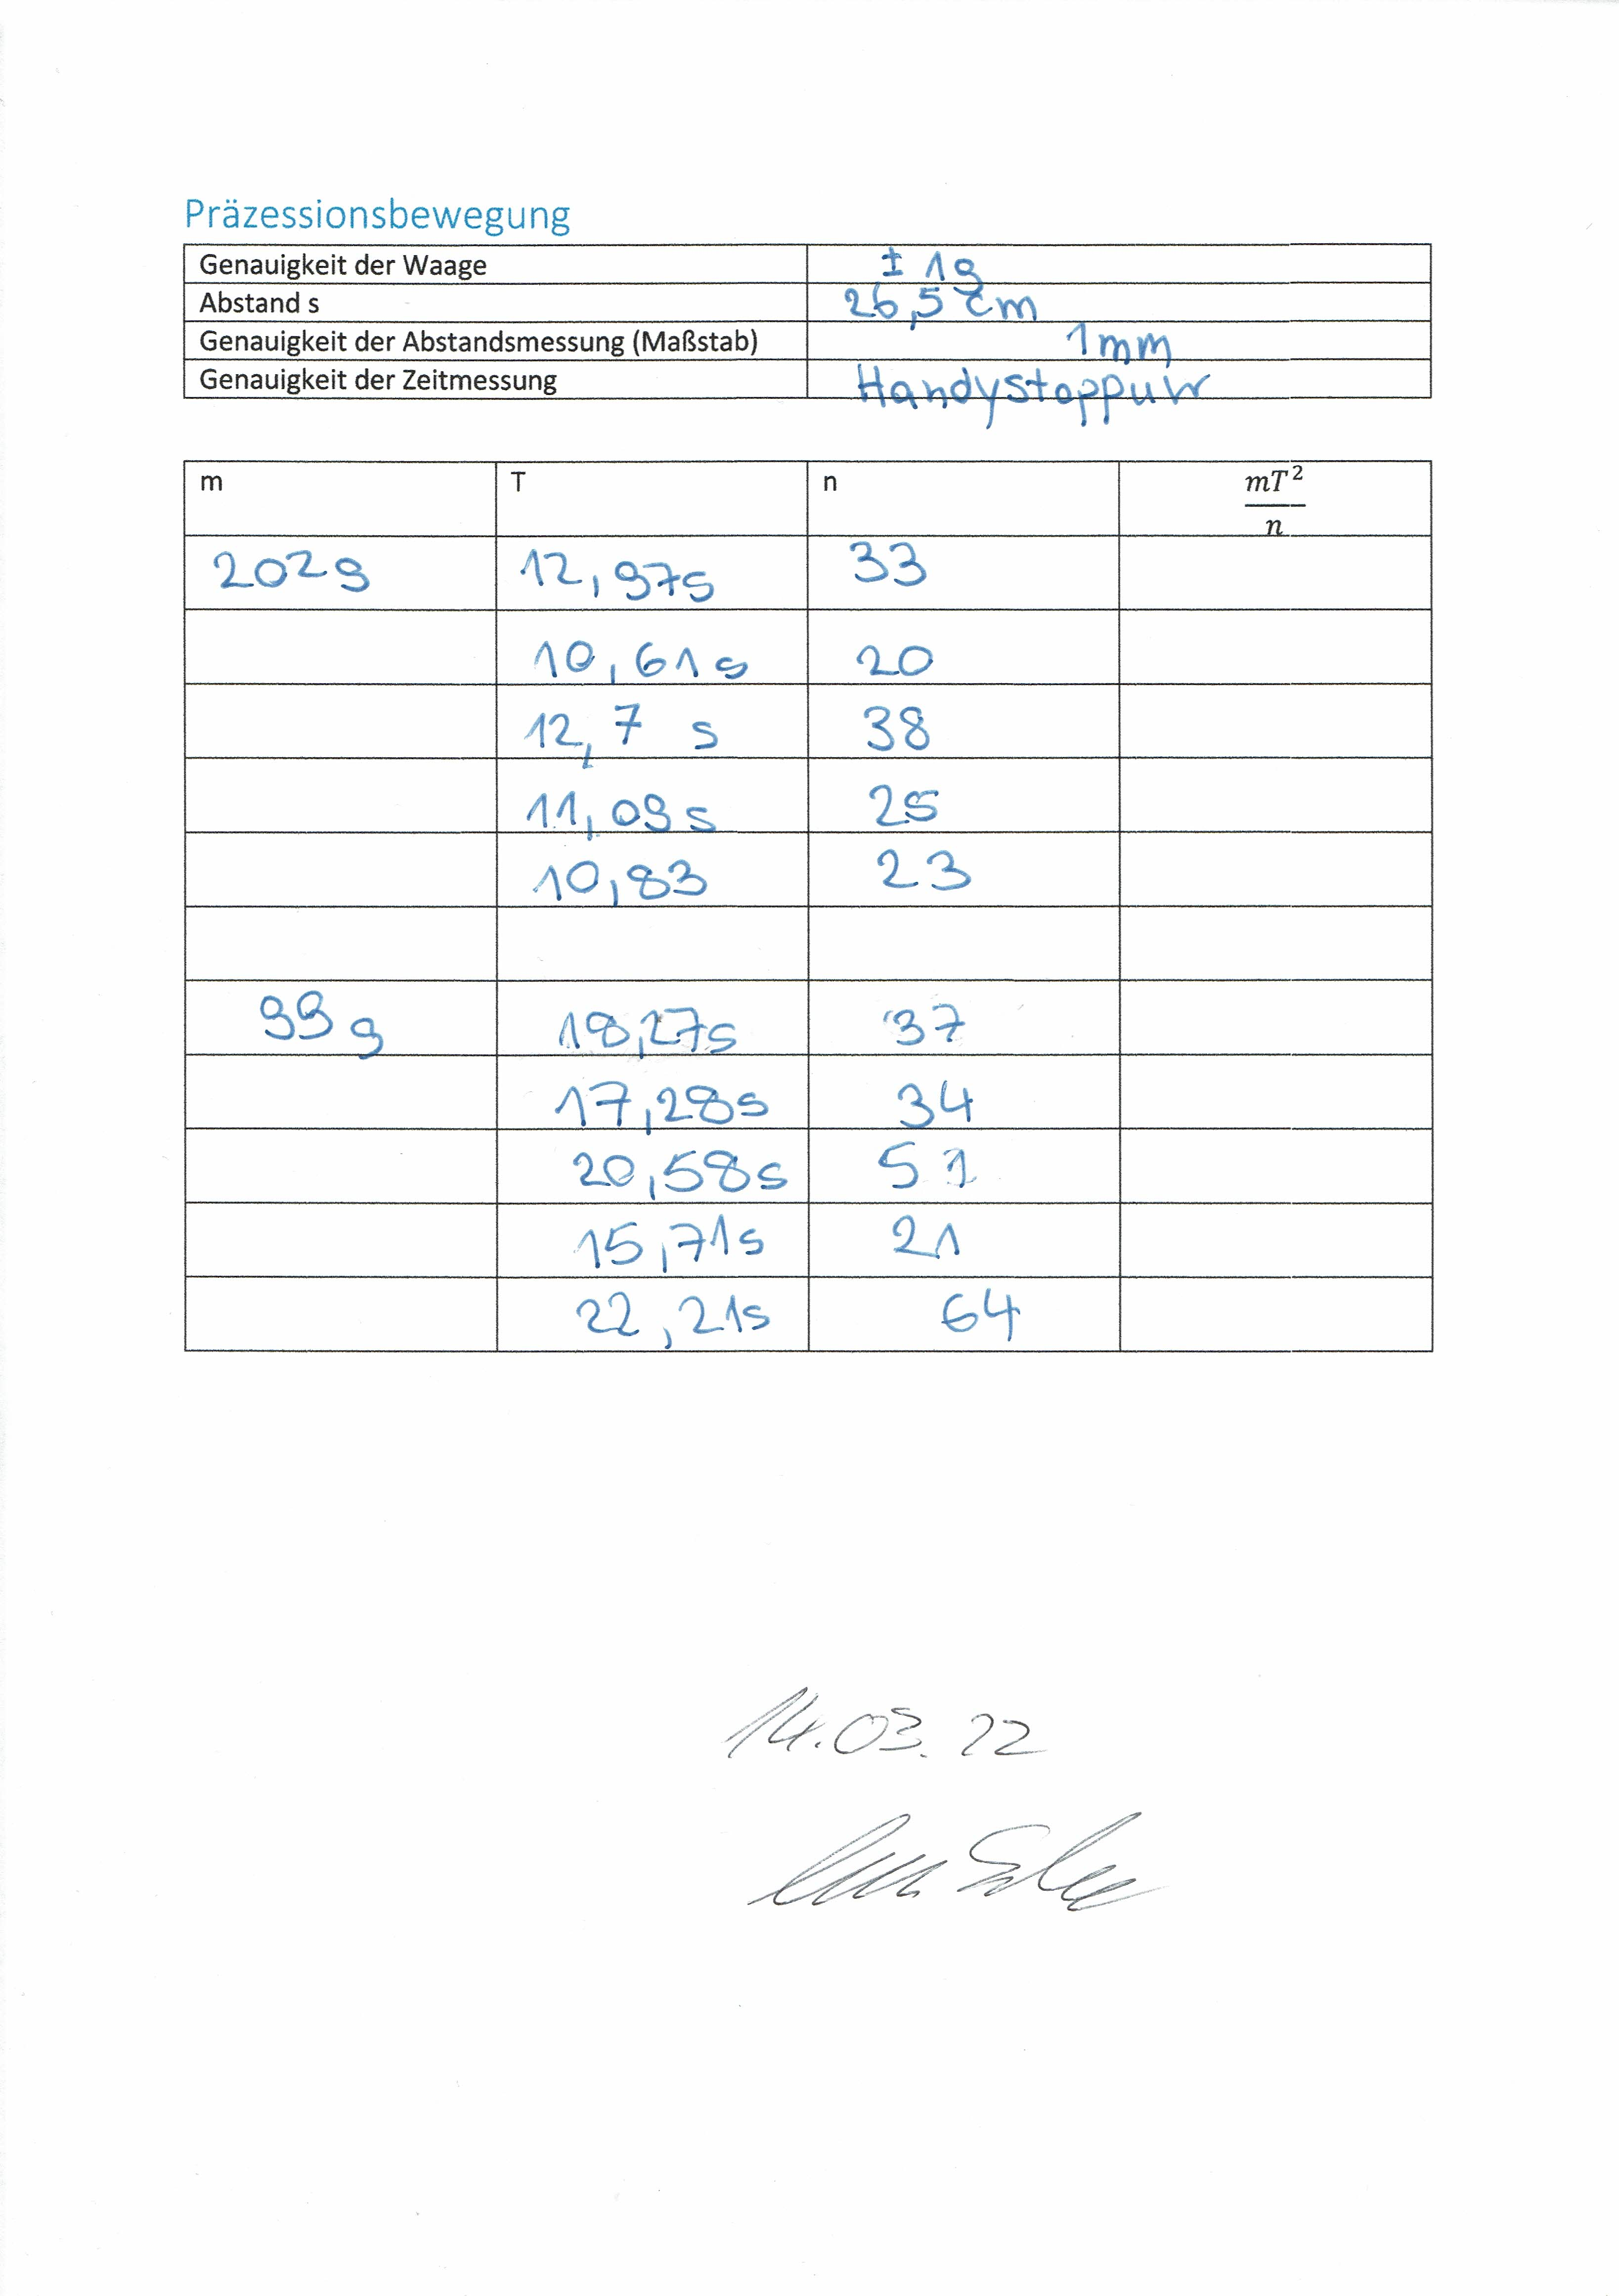
\includegraphics[height=14cm]{messwerte2.jpg}
		\caption{Messwerte des letzten Teilversuchs}
	\end{figure}

\end{document}